\chapter{Ethische Bedenken bei Algorithmen}

\section{Allgemeine Bedenken}
\begin{wrapfigure}{r}{0.5\textwidth}
	\vspace{-\baselineskip}
	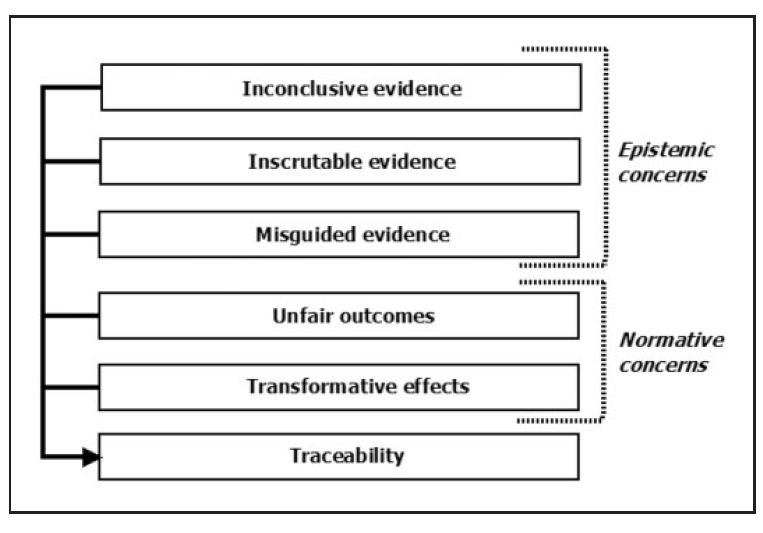
\includegraphics[width=0.48\textwidth]{resources/ethical_concerns.png}
	\caption{Sechs Arten von Bedenken \\ \cite[S. 4, Figure 1]{Sagepub2016}}
	\label{fig:Ethische Bedenken}
\end{wrapfigure}
Im Rahmen dieser Arbeit stießen die Autoren auf das Paper \citetitle{Sagepub2016} von \citeauthor{Sagepub2016}. In diesem werden verschiedene ethische Bedenken von verzerrten Algorithmen in sechs Gruppen klassifiziert. Die lauten:
\begin{itemize}
	\item Uneindeutige Anhaltspunkte
	\item Undurchsichtige Anhaltspunkte
	\item Fehlgeleitete Anhaltspunkte
	\item Unfaire Ergebnisse
	\item Transformative Effekte
	\item Nachverfolgbarkeit
\end{itemize}

Diese sechs Kategorien werden in zwei Gruppen eingeteilt: Zum Einen die epistemischen Bedenken, also jene die sich auf den Erkenntnisgewinn durch Algorithmen beziehen, zum Anderen die normativen Bedenken, deren Bewertung Teil eines gesellschaftlichen Aushandlungsprozesses ist.

\subsection{Uneindeutige Anhaltspunkte}
 Künstliche Intelligenzen und allgemein Algorithmen des maschinellen Lernens ziehen viele Schlussfolgerungen auf Grundlage von Wahrscheinlichkeiten und statistischen Mitteln.
 Deshalb sind die Ergebnisse zwar überprüfbar, aber mit Unsicherheit versehen.
 Das ist auch problematisch da häufig statistische Korrelationen benutzt werden. Aber Korrelation ist nicht gleich Kausalität - nur weil zwei Sachen immer im gleichen Kontext auftaucht, bedingen diese sich nicht gegenseitig.
 Häufig wird solche Software in einem Kontext eingesetzt in der zuverlässige Techniken und Daten entweder nicht verfügbar sind, oder zu aufwändig zu implementieren wären. Dies sollte beachtet werden, wenn aus den Ergebnissen von Algorithmen Erkenntnisse gewonnen werden sollen. 


\subsection{Undurchsichtige Anhaltspunkte}

 Als zweiten Faktor neben statistischen Mitteln, die die Ergebnisse von Algorithmen verzerren, werden in dem Paper Parameter genannt. Die Parameter eines Algorithmus können ebenfalls die Wahrscheinlichkeiten von einem Ergebnis beeinflussen. Ein großes Problem hierbei ist, dass der Zusammenhang zwischen Daten und Ergebnis häufig nicht öffentlich zugänglich. Hilfreich wäre die Zusammenhänge zwischen einzelnen Daten, sowie Parametern und deren Ergebnissen in einer Erklärung zu veröffentlichen. Allerdings ist die Funktionalität eines Algorithmus meistens ein Geschäftsgeheimnis, da man diese nicht erklären kann, ohne den Algorithmus selbst zu veröffentlichen. 
 Dies liegt in der Natur der Sache: Algorithmen sind die Beschreibung zur Abarbeitung einer Teilaufgabe. Also, wie soll man dir Beschreibung beschreiben, ohne zu viel zu verraten, aber gleichzeitig genug, um Vetrauen zu schaffen? 
 Sozusagen entstehen ethische Bedenken, wenn Algorithmen in eine BlackBox agieren. 
 

\subsection{Fehlgeleitete Anhaltspunkte}
Häufig wird als Begründung für Automatisierungen argumentiert, Software biete mehr Neutralität als menschliche Entscheidungen. Damit wird impliziert, Maschinen könnten nicht verzerrt Handeln, ohne zu bedenken, dass Maschinen, Software und Algorithmen von Menschen entworfen werden. Sie sind nicht von Natur aus neutral. Das Design und die Funktionalität von Software reflektiert Werte und Normen des Autors, allein schon durch das Prinzip der vorgesehenen Verwendung. Auch Entwicklung selbst ist kein neutraler Prozess, selten gibt es die objektiv richtige Entscheidung. Viele Entscheidungen werden auch unterbewusst getroffen. Es ist schwer Verzerrung in bestehenden Algorithmen und Modellen zu finden: Sie kann durch bereits existierenden soziale Werte, der eigenen Kultur oder Organisation, technischen Einschränkungen -- zum Beispiel vergangenen Design-Entscheidungen -- oder anderen Aspekten des Nutzungskontextes entstehen.

\subsection{Unfaire Ergebnisse}

Die vorherigen drei Bedenken beschäftigten sich mit dem Erkenntnisgewinn eines Algorithmus. Die ethischen Bedenken können jedoch auch erst beim Resultat entstehen. Vor allem dann, wenn Handlungen auf ein Ergebnis eines Algorithmus folgen, können diese ethisch unterschiedlich bewertet werden. Diese Bewertung kann man unter dem Wort "Fairness" zusammenfassen. 
So kann ein Ergebnis von einer diskriminierten Gruppe als unfair betrachtet werden, allein weil eine andere Klasse von Menschen bevorteilt wird. 
Als ein Beispiel für (un)faire Handlung aufgrund von Ergebnissen von Algorithmen, sind Vorschläge zu Berechnung von Krankenkassenbeiträge. Die erste Variante schlägt vor, dass Mitglieder mit schlechten Gesundheitswerten und wenig Eigeninitiative mehr als den Grundsatz bezahlen. Die andere Variante hingegen, dass Mitglieder mit guten Gesundheitswerten und viel Eigeninitiative einen Rabatt bekommen. 
Die Umfrage während des Vortrages hat ergeben, dass die zweite Variante höchstwahrscheinlich eher akzeptiert wird, auch wenn diese Variante ebenfalls als unfair betrachtet werden könnte.


\subsection{Transformative Effekte}
Ergebnisse von Algorithmen haben Auswirkungen auf die gesellschaftliche Wahrnehmung der Realität und beeinflussen soziale und politische Ordnungen. Sie können nachfolgende Aktionen selbst auslösen oder motivieren. Dabei besteht die Gefahr, dass eine Fehlinterpretation von Daten zu einer negativen Beeinflussung oder Beurteilung führt.

\subsection{Nachverfolgbarkeit}
Algorithmen sind Werkzeuge um große Datenbestände zu erschließen und verändern. Dadurch sind Schäden durch Algorithmen schwer zu verstehen oder nachzuvollziehen. Auch die Verantwortlichkeit oder Ursache für Schäden ist häufig ungeklärt.

\section{Verzerrte Algorithmen}

Verzerrte Algorithmen lassen sich in drei soziale Problemfelder einteilen, da nicht alle unfairen Ergebnisse eines Algorithmus den gleichen Einfluss auf unser Leben haben. 
Diese sind Entscheidungsalgorithmen, Empfehlungsalgorithmen, wie Kaufempfehlungen und Life-Style-Software.


\subsection{Entscheidungsalgorithmen}
Unter Entscheidungsalgorithmen versteht man die automatisierte Entscheidung über beispielsweise die Vergabe eine Kredites durch einen Algorithmus. In diesem Bereich gibt es einige Beispiele von verzerrte Algorithmen. 

\subsubsection{SCHUFA}
Die SCHUFA (Schutzgemeinschaft für allgemeine Kreditsicherung, Wiesbaden) ist ein Unternhemen, welches für Personen einen Score berechnet um die Kreditwürdigkeit abzubilden. Dieser Score wird anhand von verschiedenen Parametern bestimmt. Neben bereits existierenden Krediten oder Anzahl der Kontenüberziehung wird ebenfalls der Wohnort der Person in die Berechnung mit einbezogen. \newline

“Rein statistisch ist es tatsächlich unwahrscheinlicher, von jemandem, der in einem 150-Parteien-Hochhaus mit vielen Schuldnern lebt, einen Kredit zurückzubekommen“
[Thomas Riemann, Welt, 20.05.15 Geschäftsführer “Verband der Wirtschaftsauskunfteien”]

In vielen Fällen kann es dazu führen, dass der Score schlechter ausfällt, da er auch von statistischen Mitteln abhängt. \cite{welt2015}


Die Analyse einer Person anhand Ihrer Umgebung und Eigenheiten nennt man Profiling. 

\subsubsection{Profiling}
Profiling Algorithmen erkennen Korrelationen und machen Vorhersagen über Verhalten auf Gruppen-Ebene. Nutzer werden anhand von Verbindungen zu anderen Nutzern verglichen, anstatt das tatsächliche Verhalten von Individuen zu bewerten. Der Handlungsrahmen einer Person wird anhand von Informationen zur Personen-Gruppe abgesteckt. Es ist deshalb sehr naheliegend, dass diese Art von Algorithmen zu Diskriminierung neigt. Datenbasierte Benachteiligung ist genauso wenig zu ertragen wie soziale Diskriminierung aufgrund von Vorurteilen. 

\subsection{Empfehlungsalgorithmen}

% * <Alena Schemmert> 17:07:27 23 Sep 2019 UTC+0200:
% Muss noch geschrieben werden

\subsection{Life-Style-Software}
Unter Life-Style-Software verstehen wir Technologien, die uns das Leben vereinfachen sollen. Aber auch hier kann das Gegenteil eintreten, wenn die Software nicht immer wie angepriesen funktioniert. 
Ein Beispiel dafür ist ein Seifenspender welcher mit einer Künstlichen Intelligenz ausgestattet wurde. Dieser steht angeblich im Facebook Hauptbüro. 
Der Seifenspender soll automatisch Hände erkennen und eine gewissen Menge Seife in die Hände geben. Allerdings erkennt dieser Seifenspender keine dunkelhäutigen Hände. \newline 
\label{fitbit}
Ein anderes Gadget welches eigentlich das Leben erleichtern soll, aber doch häufig zu einem Ärgernis werden, ist die Fitness-Tracker-App von fitbit. Die App soll einem helfen, die eigene Aktivität oder Schlafzyklen zu messen. Zusätzlich kann man die eigene Kalorienaufnahme und das eigene Gewicht mitverfolgen. Da die täglich nötige Kalorienzufuhr und Bewegung abhängig von der physischen Verfassung ist, kommt es zu einem Problem. Vor allem bei schwangeren Frauen ist eine Gewichtszunhame und eine höhere Kalorienzufuhr wichtig für die Gesundheit. Zum Ende der Schwangerschaft, nimmt die Bewegung ab. Durch die App werden diese Aktivitäten negativ bewertet, da sie darauf programmiert ist, hohe AKtivität und vermeintlich gesundes Leben mit positiven Nachrichten zu belohnen. 
Als Frau kann man in der App einstellen, wann die Regelblutung normalerweise eintritt, oder welches Verhütungsmittel genutzt wird, aber nicht, dass man zurzeit schwanger ist und somit die anstehenden Veränderungen normal und gesund sind. 
Aber anstatt dessen, werden Frauen in besonderen Umständen mit Pushnachrichten dazu angehalten, sich mehr zu bewegen um wieder abzuspecken. 
Dieses Feature wird sich seit 2008 von der Nutzer-Community immer wieder gewünscht und betrifft immerhin die Hälfte aller potenziellen Kunden. 


\subsection{Diskussion - Ist Verzerrung eine Frage mangelnder Features?}
Die Frage war bewusst als Ja-Nein-Frage formuliert, damit sich im Rahmen der Diskussion zwei Lager bilden.

Die Verneinenden argumentierten, dass Verzerrung tatsächlich im Rahmen bestimmter Anwendungen gewollt oder erwünscht sein kann und dass es häufig schwer vorherzusehen ist, in welche Richtung sich eine spezielle Implementierung entwickeln wird. Hinzu kommt, dass ein unausgereifter Marktstart bei Software durchaus üblich ist, sodass sogar der Anspruch entstehen kann, solche Probleme nachträglich zu beseitigen. Letztendlich können dann jedoch andere Features oder Wartungsaufgaben Vorrang haben.

Auf der Pro-Seite wurde hervorgebracht, dass der Ausschluss ganzer Bevölkerungsgruppen wie im Beispiel fitbit (siehe \enquote{\ref{fitbit} \nameref{fitbit}}) durch zusätzliche Features verhindert werden könnte.
